% ============================================================================
\section{Introduction}
\label{sec:intro}
% ============================================================================

Multi-teacher on-policy distillation (MOPD) trains one student with several
specialist teachers. The student samples a response, the teacher for that task
scores it token by token, and the student parameters are updated to reduce the
sampled-token reverse KL from the student to the teacher
\citep{ma2026mopdmultiteacheronpolicydistillation}. Every method must choose a
task mixture. Open-MOPD
reports that, under token-mean aggregation, a $25\times$ response-length
difference can leave instruction following with about $1\%$ of the gradient
tokens despite receiving $20\%$ of the prompts
\citep{gao2026openmopddiagnosingfixingcapability}. D$^3$-MOPD instead adapts
the mixture from the teacher-loss gap and its descent rate
\citep{sun2026d3mopd}. In both cases, the mixture determines both the objective
weights and the computation assigned to each task. Changing the mixture changes
both quantities at once.

We specify the objective weights before training and adapt the sample counts
without changing those weights. The objective is a weighted sum of per-task
teacher losses. Each optimizer step contains $G$ fixed-size micro-batches, each
from one task, and the online decision is the number assigned to each task.
Multiplying each task's micro-batch losses by its fixed weight divided by its
count preserves the expected gradient under every allocation
(Section~\ref{sec:setting}). The counts therefore affect estimator variance but
not the training objective.

Minimizing the variance of this estimator assigns more micro-batches to tasks
with larger gradient noise. Gradient-Preconditioned Adaptive Sampling (GPAS)
measures the noise after AdamW's diagonal scaling and assigns task $i$ a count
proportional to $w_i\sqrt{e_i}$. This is the classical stratified-sampling rule
that assigns samples in proportion to each stratum's standard deviation,
applied in the coordinates used for the optimizer update. Raw and scaled
gradient noise can rank tasks differently. In our controlled check, allocation
based on raw noise produces $2.316\times$ the scaled variance of Uniform,
whereas GPAS produces $0.679\times$. Cost-GPAS modifies the counts using the
measured task-specific time per micro-batch and the fixed time per optimizer
step.

\begin{figure}[t]
    \centering
    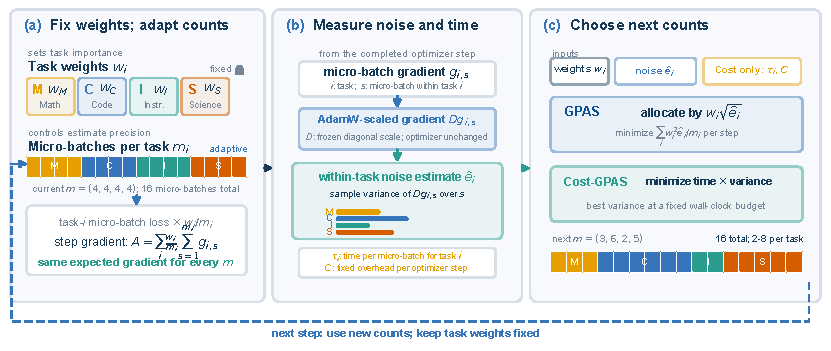
\includegraphics[width=\linewidth]{figures/gpas_main_figure.pdf}
    \caption{GPAS fixes the objective weights $w$ and adapts only the
    micro-batch counts $m$. Gradients from the completed step provide each
    task's noise in AdamW coordinates; measured time adds the cost correction.
    GPAS computes the next step's allocation without additional model passes.}
    \label{fig:gpas_overview}
\end{figure}

Computing the allocation statistics requires no additional model passes. Every
task is present in every step, so the trainer estimates within-task noise from
the gradients computed in that step and obtains timings from the same execution
trace. A minimum count keeps every teacher in every step and provides a new
noise estimate. GPAS works with conventional AdamW. We separately evaluate an
optional taskwise second-moment observation that removes allocation dependence
from AdamW's second-moment target.

The four-teacher study tests whether lower one-step gradient variance improves
training loss, compute efficiency, and downstream capability. \missing{After completing the runs, summarize here: the range
and drift of optimizer-scaled noise, the reduction in weighted teacher loss at
matched steps, the GPU-hour saving of Cost-GPAS, and whether any downstream
task regresses relative to Uniform.}

Our contributions are:
\begin{itemize}
    \item a fixed-objective MOPD estimator in which adaptive micro-batch counts
    change sampling variance but not the expected task weights;
    \item GPAS and Cost-GPAS, optimizer-aware count rules whose online
    statistics are obtained from the model passes already required by MOPD;
    \item a four-teacher evaluation of allocation dynamics, loss per optimizer
    step, loss per GPU hour, and the variance ratio relative to Uniform,
    together with reproducible controlled checks.
\end{itemize}
